\documentclass[11pt,twocolumn,nocopyright]{sigplanconf}

% The following \documentclass options may be useful:
%
% 10pt          To set in 10-point type instead of 9-point.
% 11pt          To set in 11-point type instead of 9-point.
% authoryear    To obtain author/year citation style instead of numeric.

% save and then undefine the conflicting command
% we need \makeatletter because \@undefined uses the special @ character.

\usepackage{amsthm}
\usepackage{amsmath}
\usepackage{amssymb}
\usepackage{graphicx}
\usepackage{epstopdf}
\usepackage{hyperref}
\usepackage{alltt}
\usepackage{listings}
\usepackage{array}
\usepackage{extarrows}
\usepackage{setspace}
\usepackage{tikz}
\usepackage{tikz-qtree}
\usetikzlibrary{calc}
\usetikzlibrary{positioning}
\usepackage{floatrow}
\usepackage[noline, boxed, procnumbered, linesnumberedhidden, titlenumbered]{algorithm2e} 

%\usepackage[margin=0.75in]{geometry}

%\usepackage{graphviz}
%\usepackage{gastex}

\newcommand{\cut}[1]{}

\newcommand{\sbull}{\,\begin{picture}(-1,1)(-1,-2.2)\circle*{2.2}\end{picture}\ }

\newcommand{\techreport}[1]{} % drop #1 to make it a cut
\newcommand{\todo}[1]{{\bf\em TODO:} #1}
\newcommand{\rem}[1]{{\bf\em rem:} #1}
\newcommand{\reminder}[1]{{\it #1 }}
\newcommand{\edcom}[1]{\textbf{{#1}}}
%\newcommand{\poplversion}[1]{#1}
\newcommand{\trversion}[1]{}

\newcommand{\appref}[1]{Appendix~\ref{#1}}
\newcommand{\secref}[1]{Section~\ref{#1}}
\newcommand{\tblref}[1]{Table~\ref{#1}}
\newcommand{\figref}[1]{Figure~\ref{#1}}
\newcommand{\thmref}[1]{Theorem~\ref{#1}}
\newcommand{\algref}[1]{Algorithm~\ref{#1}}
\newcommand{\funref}[1]{Function~\ref{#1}}
\newcommand{\listingref}[1]{Listing~\ref{#1}}
%\newcommand{\pref}[1]{{page~\pageref{#1}}}

\newcommand{\eg}{{\em e.g.}}
\newcommand{\cf}{{\em cf.}}
\newcommand{\ie}{{\em i.e.}}
\newcommand{\etal}{{\em et al}}
\newcommand{\etc}{{\em etc.\/}}
\newcommand{\naive}{na\"{\i}ve}
\newcommand{\role}{r\^{o}le}
\newcommand{\forte}{{fort\'{e}\/}}
\newcommand{\appr}{\~{}}

\newcommand{\llk}{{\em LL(k)}}
\newcommand{\lalrk}{{\em LALR(k)}}
\newcommand{\lalr}{{\em LALR}}
\newcommand{\LL}{{\em LL}}
\newcommand{\LR}{{\em LR}}
\newcommand{\lrk}{{\em LR(k)}}
\newcommand{\lr}{{\em LR}}
\newcommand{\llr}{{\em LL}-regular}
\newcommand{\lrr}{{\em LR}-regular}
\newcommand{\sllr}{{\em SLL}-regular}
\newcommand{\SLL}{{\em SLL}}
\newcommand{\slls}{{\em SLL(*)}}
\newcommand{\lls}{{\em LL(*)}}
\newcommand{\alls}{{\em ALL(*)}}
\newcommand{\salls}{{\em SALL(*)}}
\newcommand{\smallstate}[1]{\vspace{.4em}\mbox{\Large $\bigcirc \hspace{-0.47cm}$} \raisebox{.02em}{$#1$} }
\newcommand{\bigstate}[1]{\vspace{.4em}{\huge $\bigcirc \hspace{-0.67cm}$} \raisebox{.3em}{$#1$} }
\newcommand{\state}[1]{\bigstate{~#1~}}
\newcommand{\gpos}{\raisebox{.2em}{\,.}}
\newcommand{\store}{\mathbb{S}}
\newcommand{\cont}{\mathcal{C}}
\newcommand{\ith}{$i^{th}$}

\newcommand{\closure}{\textit{closure}}
\newcommand{\move}{\textit{move}}
\newcommand{\predict}{\textit{predict}}
\newcommand{\resolve}{\textit{resolve}}
\newcommand{\resolveWithPredicate}{\textit{resolveWithPredicate}}
\newcommand{\resolvedWithPredicate}{\textit{wasResolved}}

\newcommand{\lowerbox}[2]{$_{\mbox{#2}}$}

\newtheorem{theorem}{Theorem}[section]
\newtheorem{lemma}{Lemma}[section]
\newtheorem{definition}{Definition}[section]
\newtheorem{conjecture}{Conjecture}[section]

\newcommand{\pq}[3]{\state{#1} \hspace{-0.45em}$\xrightarrow{#2}$ \hspace{-0.8em} \state{#3}}

\toappear{}
\begin{document}

\title{Grammars: Raw lecture notes}

\authorinfo{Terence Parr\vspace{-1mm}}
           {University of San Francisco\vspace{-1mm}}
           {parrt@cs.usfca.edu}

\maketitle

\begin{abstract}
\end{abstract}

\section{CFGs}

A {\em grammar} is a set of rules that describe the set of valid sentences in a language, $L$. The rules have a very specific format and therefore follow a language, a metalanguage. The rules are called {\em production rules} and say how to generate strings in the language. There are rule names, {\em non-terminals}, and vocabulary symbols ({\em terminals} or {\em tokens}). The rules are of the form

$leftside \rightarrow rightside$

Context free grammar: {\em CFG} is a grammar where $leftside$ has to be a single non-terminal:

$expression \rightarrow {\bf id}$

there can be multiple rules

$expression \rightarrow {\bf integer}$

For formal grammars we tend to use single single capital letters for non-terminals CFG notation:

\noindent $
E \rightarrow {\bf id} \\
E \rightarrow {\bf integer}$

 examples
 
\noindent $
A \rightarrow {\bf a} \\
A \rightarrow {\bf b} \\
$

Or, $A \rightarrow {\bf a} | {\bf b}$

Language $L = \{a,b\}$.

 Infinite languages
 
 \noindent $
A \rightarrow a A \\
A \rightarrow \epsilon \\
$

or

 \noindent $
A \rightarrow a A \\
A \rightarrow \\
$

$L = {a^*}$

\noindent $
A \rightarrow a A \\
A \rightarrow a\\
$

$L = {a^+}$

Many grammars for one $L$.

A  CFG grammar $G = (N, T, P, S)$ has elements:

\vspace{-3pt}
\begin{itemize}\itemsep0pt \parskip0pt \parsep0pt
\item $N$ is the set of nonterminals (rule names)
\item $T$ is the set of terminals (tokens)
\item $P$ is the set of productions
\item $S \in N$ is the start symbol
\end{itemize}

\begin{center}\small 
\begin{tabular}{l  l}
$A  \in N$		    & Nonterminal \\
$a,b,c,d  \in T$ 	    & Terminal \\
$X  \in (N \cup T)  $ & Production element \\
$\alpha, \beta, \delta \in X^*$  & Sequence of grammar symbols\\
$u,v,w,x,y \in T^*$             & Sequence of terminals\\
%$w_r \in T^*$             & Remaining input terminals\\
$\epsilon$ & Empty string \\
$\char36$ & End of file ``symbol'' \\
\end{tabular}
\end{center}


$L = \{a^nb^n | n \ge 1\}$ is CF but $L = \{a^nb^nc^n | n \ge 1\}$ non CF.

\noindent $
A \rightarrow a A b\\
A \rightarrow a b\\
$

The set of all context-free languages is identical to the set of languages accepted by pushdown automata ({\em PDA}) and all contexts we languages can be parsed in $O(n^3)$ time.

\section{Regular grammars}. A single non-terminal on the left like CFG, but the right-hand side can only be: empty, a sequence of terminals, a sequence of terminals followed by a non-terminal, but that's it. All regular languages can be recognized by a finite state machine linear time. NFA/DFA.

Non-regular $\{a^nb^n | n \ge 1\}$ because we have no memory but $\{a^nb^m | n \ge 1\}$ is regular.

\noindent $
A \rightarrow a^* b^*\\
$

\section{EBNF}

which introduces us to extended BNF (EBNF). we typically use a variation on {\tt yacc} notation, which flips things so that non-terminals are lowercase and terminals are uppercase like constants:

\begin{alltt}
a : A* B* ; // extended; yacc doesn't allow *
\end{alltt}

or

\begin{alltt}
a : 'a'* 'b'* ; // ANTLR notation
\end{alltt}

\begin{alltt}\small
grammar Ex; // generates class ExParser
// action defines ExParser member: enum_is_keyword
@members \{boolean enum_is_keyword = true;\}
stat: expr '=' expr ';' // production 1
    | expr ';'          // production 2
    ;
expr: expr '*' expr
    | expr '+' expr
    | expr '(' expr ')' // f(x)
    | id
    ;
id  : ID | \{!enum_is_keyword\}? 'enum' ;
ID  : [A-Za-z]+ ; // match id with upper, lowercase
WS  : [ \textbackslash{}t\textbackslash{}r\textbackslash{}n]+ -> skip ; // ignore whitespace
\end{alltt}

\section{Derivations}

$\alpha \Rightarrow \beta$ $\alpha \Rightarrow^* \beta$ $\alpha \Rightarrow^+ \beta$

how to regenerate a string starting from the start symbol?

\noindent $
A \rightarrow a A b\\
A \rightarrow a b\\
$

generation of $ab$:
 
$A \Rightarrow ab$

generation of $aabb$:
 
$A \Rightarrow aAb \Rightarrow aaba$

leftmost and rightmost derivations
 
\noindent $
S \rightarrow {\bf if} E {\bf then} S\\
S \rightarrow {\bf return} E\\
E \rightarrow {\bf id}\\
$

$S \Rightarrow_{lm} {\bf if} E {\bf then} S \\
\Rightarrow_{lm} {\bf if} {\bf x} {\bf then} S \\
\Rightarrow_{lm} {\bf if} {\bf x} {\bf then} {\bf return} E \\
\Rightarrow_{lm} {\bf if} {\bf x} {\bf then} {\bf return} {\bf y}$

or

$S \Rightarrow_{rm} {\bf if} E {\bf then} S \\
\Rightarrow_{rm} {\bf if} E {\bf then} {\bf return} E \\
\Rightarrow_{rm} {\bf if} E {\bf then} {\bf return} {\bf y}\\
\Rightarrow_{rm} {\bf if} {\bf x} {\bf then} {\bf return} {\bf y}$

diff deriv but same tree. So parse tree of $A$ then if-then-else.

Formally, the language generated by grammar sequence $\alpha$ in user state $\store$ is
$L(\alpha)=\{ w \, | \, (\alpha) \Rightarrow^*
(w)\}$ and the language of grammar $G$ is $L(G) = \{ w \, | \,
(S) \Rightarrow^* (w)\}$. Language $L$ is CF {\em iff} there exists a CFG for $L$.

$\alpha$ is {\em sentential form} if S derives to it. If $\alpha \in T \cup N$ it's a {\em sentence}.

Proof that $G$ gens $L$ means show every string gen'd by G is in L and every string in L can be gen'd by G. and

\section{Parse trees}

Show parse tree of  $A \rightarrow a A | \epsilon$ and if-then-else above.

\section{Ambiguity}

See section 5.4 in ANTLR 4 book. p69 printed.

more than one lm or rm deriv for same input. normally an error. $L$ can be ambig too syntactically; e.g., expressions. Ambig $L$ gives ambig $G$. Need disambiguating rules from semantics or otherwise.

\noindent $
A \rightarrow a A | \epsilon \\
$
classic:

\noindent $
E \rightarrow E * E\\
E \rightarrow E + E\\
E \rightarrow {\bf id}\\
$

1+2*3 has two interps. show trees.

Parse trees for {\tt a*b+c} and $E \rightarrow E * E \,|\, E {\bf +} E \,|\, {\bf id}$. Converted to non-Left-recur:  $E \rightarrow {\bf id}\ (*\ E | {\bf +}\ E)^*$. The parser must recognize {\tt a*b+c} as {\tt (a*b)+c} not {\tt a*(b+c)}.

\begin{center}
\begin{small}
\begin{tabular}{cc}
\scalebox{.9}{
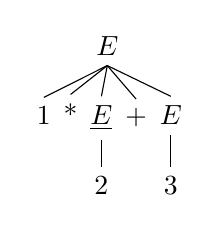
\begin{tikzpicture}
\tikzset{level distance=25pt, sibling distance=-2pt}
\Tree
[.$E$
  1 * [.$\underline{E}$ 2 ] +  [.$E$ 3 ]]
]
\end{tikzpicture}
} & \scalebox{.9}{
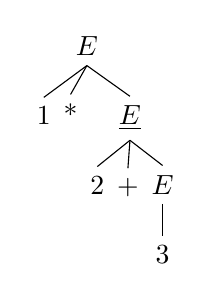
\begin{tikzpicture}
\tikzset{level distance=25pt, sibling distance=-2pt}
\Tree
[.$E$
  1 *
  [.$\underline{E}$ 2 + [.$E$ 3 ]]
]
\end{tikzpicture}
} \\
{\bf (a)} {\tt (a*b)+c} & {\bf (b)} {\tt a*(b+c)} \\
\end{tabular}
\end{small}
\end{center}


A predicated grammar $G = (N, T, P, S, \Pi, \mathcal{M})$ has elements:

\begin{itemize}\itemsep0pt \parskip0pt \parsep0pt
\item $N$ is the set of nonterminals (rule names)
\item $T$ is the set of terminals (tokens)
\item $P$ is the set of productions
\item $S \in N$ is the start symbol
\item $\Pi$ is a set of side-effect-free semantic predicates
\item $\mathcal{M}$ is a set of actions (mutators) 
\end{itemize}

\section{Left recur}

Indirectly left-recursive rules call themselves through another rule; e.g., $A
\rightarrow B$, $B \rightarrow A$. Hidden left-recursion occurs
when an empty production exposes left recursion; e.g., $A \rightarrow
B A$, $B \rightarrow \epsilon$.

\noindent $
A \rightarrow A a\\
A \rightarrow b\\
$

right recur

\noindent $
A \rightarrow a A\\
A \rightarrow b\\
$

Ex: elim in direct left recur

\noindent $
E \rightarrow E * E\\
E \rightarrow E / E\\
E \rightarrow E + E\\
E \rightarrow {\bf id}\\
$

Show typical non-left recur arith expr rules.

\section{Left factoring}

\noindent $
S \rightarrow {\bf if} E {\bf then} S {\bf else} S\\
S \rightarrow {\bf if} E {\bf then} S\\
$

\noindent $
S \rightarrow {\bf if} E {\bf then} S S'\\
S' \rightarrow {\bf else} S \\
S' \rightarrow
$

or EBNF

\noindent $
S \rightarrow {\bf if} E {\bf then} S ({\bf else} S)^?\\
$


\end{document}